\chapter{State Estimation}
\label{ch:estimation}
One of the ACS libraries is the extended Kalman filter which is used on the EOD robots for state estimation and is the main method used for answering the question ``Where am I?''. The idea behind the Kalman filter is relatively straightforward in that the robot has some basic idea of where it is in the world using its sensors but there is uncertainty involved in that estimate due to:
\begin{itemize}
\item different measurement accuracies from the sensors,
\item multiple sensors measuring the same state,
\item some states that are not measured,
\item imperfect models of the robot dynamics.
\end{itemize}

The Kalman filter is a method to merge physical models and sensor data to come up with an estimate of where the robot is located, what its orientation is and how fast it is moving that is better than any of the individual sensor measurements \cite{Simon06OptimalEstimation}, \cite{Grewal08}, \cite{Orderud05}. There are four models used in the Kalman filter:
\begin{itemize}
\item system model based on physics,
\item measurement model to transform sensor output to state coordinate system,
\item system noise model,
\item measurement noise model.
\end{itemize}

\section{State Space Models}
\label{sec:statespacemodels}
Kalman filters and modern control systems (see Chapter \ref{ch:controls}) use the idea of a multi-dimensional state space to encapsulate all of the relevant information that is known about a system. In the case of robots like the ones used in these experiments the states of interest are position, orientation and linear and angular velocities. In general a system is described by nonlinear equations that describe how the state variables change through time and how measurements of the system are related to the states as given by
\begin{align}
\label{eq:statespace}
\begin{split}
\dot{x} &= f(x,u,t) \\
\dot{y} &= h(x,t).
\end{split}
\end{align}

The state variables are given in vector form by $x$ and the sensor measurements are contained in the vector $y$. The state space equations are a means of representing with compact notations how the state of a system changes through time based on the initial state of the system and the inputs to the system, $u$, which allows the trajectory (or motion through time) to be calculated. The inputs are assumed to include any external forces applied to the system as well as actuation provided by the system itself. The function $h(x,t)$ transforms the sensor measurements into state variables.

For the robots used in these experiments the state vector used follows that found in \cite{Kelly_1994_338}, \cite{Kelly_1994_333} where the state variables are
\begin{align*}
x_k = \left[\begin{array}{c c c c c c c c} x & y & z & V & \theta & \phi & \psi & \omega \end{array}\right]^T.
\end{align*}
In this vector $x$, $y$ and $z$ are positions, $V$ is linear velocity, $\theta$, $\phi$ and $\psi$ are Euler angles for pitch, roll and yaw, and $\omega$ is angular velocity as shown in Figure \ref{fig:packbotaxes}.

\begin{figure}[ht!]
    \centering
    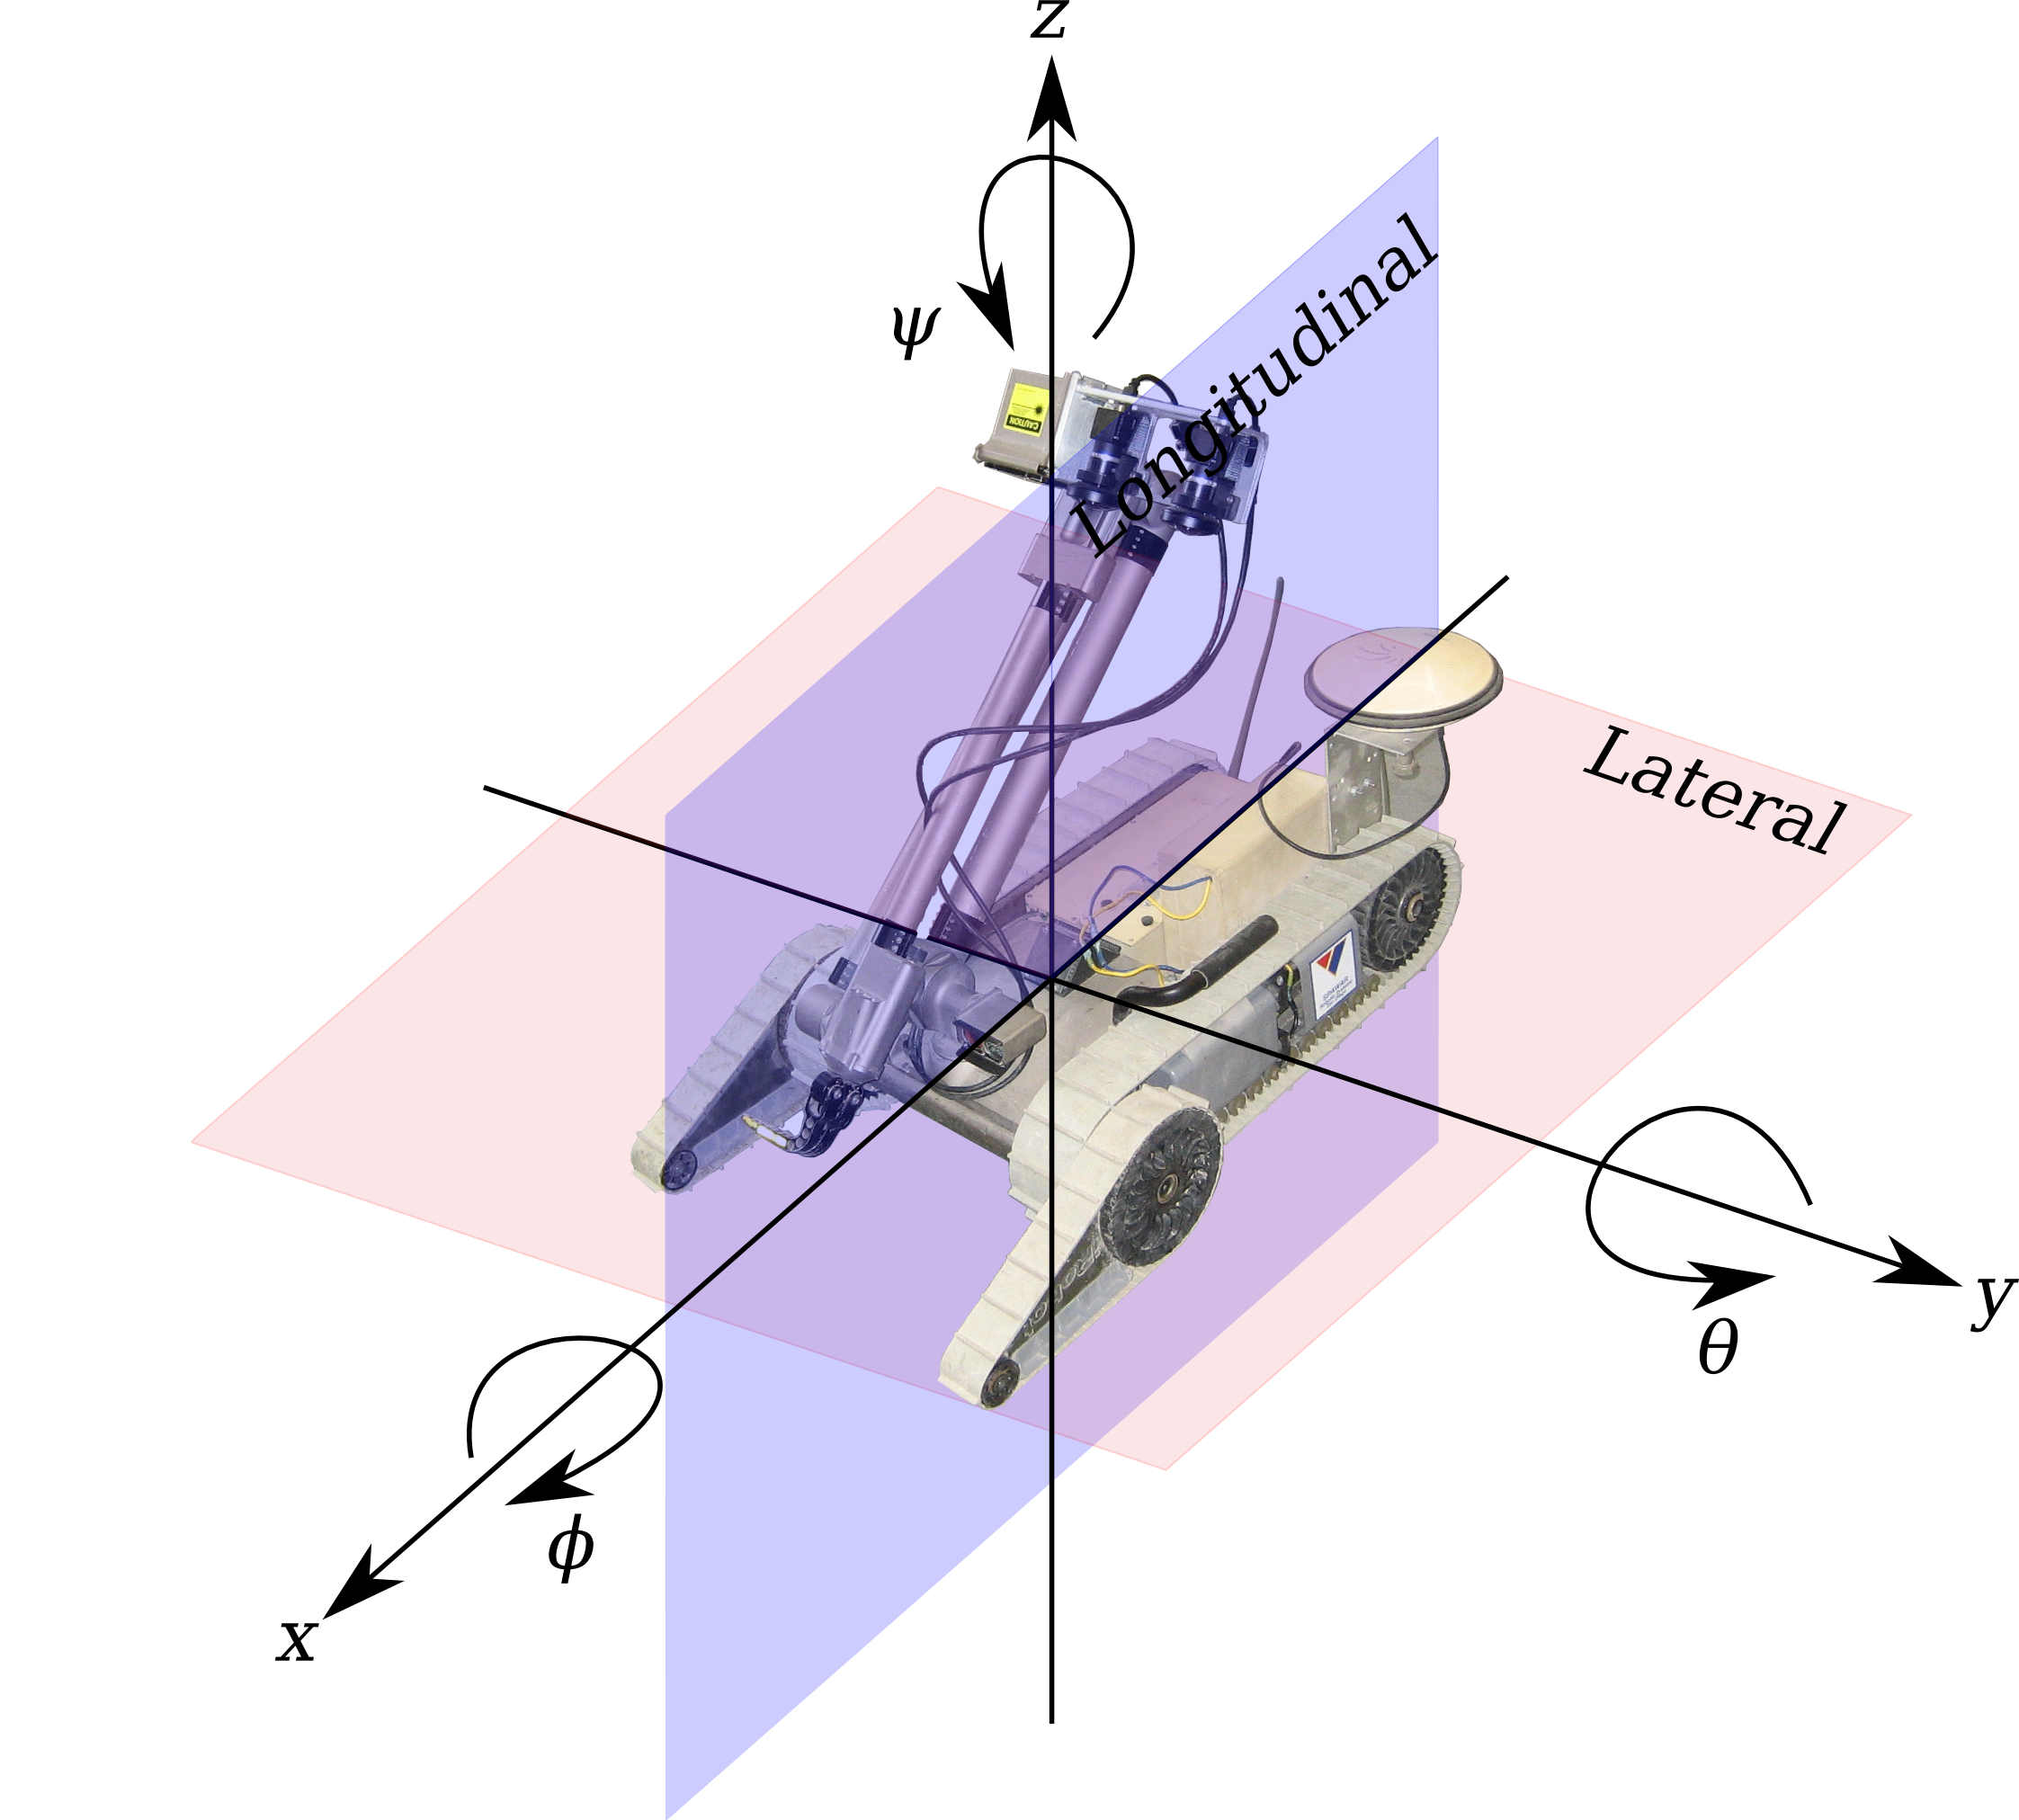
\includegraphics[width=.8\textwidth]{images/packbotaxes}
    \caption{PackBot Axes for Position and Orientation}
    \label{fig:packbotaxes}
\end{figure}

\section{The Kalman Filter}
\label{sec:kalmanfilter}
The ACS Kalman filter is typical of all Kalman filters in that it consists of a prediction update step and a measurement update step where the prediction update is run as fast as possible and the measurement update is run whenever new sensor data becomes available as depicted in the block diagram of Figure \ref{fig:kf}. The prediction update step uses a model of the system dynamics and a measurement of elapsed time to determine where the system is in the world and will inevitably have errors. Some of the errors are due to effects that are not captured in the models, (im)precision of the clock on the computer for measuring time and simplifying assumptions that are made in order to be able to calculate the system model in real-time using embedded computers. The measurement update step is basically a feedback step to help correct for errors in the system model using sensors to provide current data \cite{Kelly_1994_338}.

\begin{figure}[ht!]
	\centering
	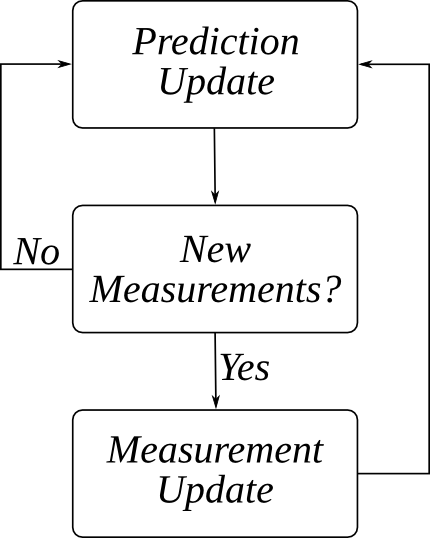
\includegraphics[width=.4\textwidth]{images/kf}
	\caption{The Kalman Filter Algorithm}
	\label{fig:kf}
\end{figure}

The Kalman filters that run on the small UGVs used in these experiments run on digital computers and are necessarily used in discrete time rather than continuous time because of the nature of computers. Additionally, the standard Kalman filter equations make the assumption that the system and measurement models are linear. From \cite{Kelly_1994_338}, \cite{Simon06OptimalEstimation} the discretized and linearized versions of (\ref{eq:statespace}) mean that the state space equations are represented as
\begin{align*}
%\label{eq:kfstatemodel}
\begin{split}
x_{k+1} &= \Phi_kx_k + w_k \\
y_k &= H_kx_k + v_k
\end{split}
\end{align*}
where $\Phi_k$ is the discrete time state transition matrix relating the state at time $k+1$ to time $k$ in the absence of inputs or noise and models the system dynamics, $w_k$ is system noise due to an imperfect model, $H_k$ is the measurement matrix which relates the measurements to the state vector and $v_k$ is the sensor measurement noise. The ACS Kalman filter uses an unforced model so all inputs are considered disturbances to the steady-state dynamics. This means that $w_k$ includes noise, modeling errors, external forces and actuator forces.

The prediction update step marches the system dynamics forward in time using the equations
\begin{align}
\label{eq:kfpredictionupdate}
\begin{split}
\hat{x}_{k+1}^- &= \Phi_k\hat{x}_k^+ \\
P_{k+1}^- &= \Phi_kP_k^+\Phi_k^T + Q_k
\end{split}
\end{align}
and the measurement update step provides feedback from sensor data using the equations
\begin{align}
\label{eq:kfmeasurementupdate}
\begin{split}
K_k &= P_k^-H_k^T\left[H_kP_k^-H_k^T + R_k\right]^{-1} \\
\hat{x}_k^+ &= \hat{x}_k^- + K_k\left[y_k - H_k\hat{x}_k^-\right] \\
P_k^+ &= \left[I - K_kH_k\right]P_k^-
\end{split}
\end{align}
where $P_k$ is the state covariance matrix, $K_k$ is the Kalman gain, $Q_k = E[w_kw_k^T]$ is the process covariance matrix giving a measure of the expected noise in the system model and $R_k = E[v_kv_k^T]$ is the measurement covariance matrix giving the expected noise of the sensors. Using (\ref{eq:kfpredictionupdate}) and (\ref{eq:kfmeasurementupdate}) an estimate of the state of the robot can be obtained at any time for use by the controls algorithms, to give feedback to a human operator or to share with other systems that can change their behavior based on the state of the robot.

The variables $\hat{x}_k^-$, $P_{k+1}^-$ in (\ref{eq:kfpredictionupdate}) and $\hat{x}_k^+$, $P_{k}^+$ in (\ref{eq:kfmeasurementupdate}) refer to estimates and covariances of the state variables before and after the measurement update step in the Kalman filter, respectively. Each of the terms in the Kalman filter equations is discussed in more detail in subsequent sections.

\subsection{Models in the Kalman Filter}
\label{sec:kfModels}
The Kalman filter relies on several models that are used to determine estimates and covariances of the states for a system. The ACS Kalman filter uses four such models:
\begin{itemize}
\item System dynamics model $\Phi_k$,
\item measurement model $H_k$,
\item system noise model $Q_k$,
\item measurement noise model $R_k$.
\end{itemize}

It is important to recognize that the fidelity of and interaction between these four models determines how well the Kalman filter output will represent the true state of the robot.

\subsection{Assumptions in the System Model}
\label{sec:kfAssumptions}
It is nearly impossible to develop models that completely capture all of the attributes of most systems, including robots that are expected to operate in many different physical environments, so assumptions are made to simplify the system model. The following assumptions allow the prediction update step to be calculated in a reasonable amount of time using modern computers so that a state estimate is available that the control systems can act upon in real time. The assumptions also allow a single system model to be abstracted and used on multiple similar but different robotic vehicles such as those described in Chapter \ref{sec:smallugvs}.

\subsubsection{Low Dynamics Assumption}
\label{sec:kfLowDynamicsAssumption}
The first assumption made is that, from one time step to the next, the robot will not be accelerating fast enough in any direction for the sensors on the robot to be able to measure the accelerations. This means that the two velocities, linear and angular, in the state vector will be assumed to be constant. The benefit of this assumption is that there are six fewer states that must be tracked in the state vector, one for acceleration about each axis of the robot.

\subsubsection{Principal Motion Assumption}
\label{sec:kfPrincipalMotionAssumption}
The second assumption says that, during a single time step, the position of the robot will only be a function of linear velocity and the orientation of the robot will only be a function of the angular velocity. Figure \ref{fig:packbotaxes} helps in visualizing the effect of rotating the robot about its center and how that will not affect the position of the robot. Similarly, tranlation of the robot along the $x$, $y$ or $z$ axis will not change the orientation of the robot. This assumption allows several terms in the system model to be set to zero.

\subsection{Continuous to Discrete Time Transform}
\label{sec:kfContToDiscTransform}
The system model will initially be developed using continuous time nonlinear differential equations but the Kalman filter on the robots will be running on digital computers so the model will need to be converted to discrete time. In continuous time the system model will be
\begin{align*}
\dot{x} = Fx
\end{align*}
and in discrete time the system model will be
\begin{align*}
x_{k+1} = \Phi_k x_k.
\end{align*}
The transformation from continuous to discrete time obeys an exponential matrix transformation with a Taylor series approximation \cite{Gelb74} given by
\begin{align*}
\Phi_k = e^{F\Delta_T} = I + F\Delta_T + \frac{(F\Delta_T)^2}{2!} + \ldots + \frac{(F\Delta_T)^n}{n!}
\end{align*}
A first order Taylor series approximation is generally considered good enough when $\Delta_T$ is small and if the nonlinearities in the system are small enough. In the case of the robots used in these experiments that is assumed to be the case so the transformation used is simply
\begin{align}
\label{eq:kfContToDiscTransform}
\Phi_k = I + F\Delta_T.
\end{align}

\subsection{System Dynamics Model}
\label{sec:dynamics}
A model of the system dynamics is necessary in order to propagate the state of the system forward in time in the absence of measurements. It is impossible to create a perfect model of the system and even a nearly perfect model of the system will likely be too complex to compute fast enough for it to be useful. The best result that is typically available is a model with a large amount of assumptions where the most important aspects of the dynamics are captured in the model.

A nonlinear, continuous time model based on robot kinematics is developed in the body frame coordinate system using the states from Chapter \ref{sec:statespacemodels} is given by
\begin{align}
\label{eq:kfnonlineardynamics}
\begin{split}
\frac{d}{dt}\left[\begin{array}{c}
x \\ y \\ z \\ V \\ \theta \\ \phi \\ \psi \\ \omega
\end{array}\right] =
\left[\begin{array}{c}
V\cos\psi\cos\theta \\
V\sin\psi\cos\theta \\
-V\sin\theta \\
0 \\
-\omega\sin\phi \\
\omega\tan\theta\cos\phi \\
\omega\cos\phi/\cos\theta \\
0
\end{array}\right].
\end{split}
\end{align}

\subsection{Extended Kalman Filter}
\label{sec:extendedkf}
The basic Kalman filter makes the assumption that both the system model contained in $\Phi_k$ and the measurement model in $H_k$ are linear. The extended Kalman filter (EKF) allows for nonlinear models such as that given by (\ref{eq:kfnonlineardynamics}) to be used for $\Phi_k$, $H_k$ or both by linearizing the models around the state estimate. To linearize the models the Jacobian, or matrix of partial derivatives, is taken about the estimated state. The idea of linearization of a nonlinear model is shown in Figure \ref{fig:KFLinearization} where the linearization can be seen to be more accurate when the system nonlinearities are small meaning that the dynamics are slow.

\begin{figure}[ht!]
	\centering
    \subfloat[Slow dynamics.] {
	    \label{images/KFLinearizationSlow}
        \includegraphics[width=.3\textwidth]{images/KFLinearizationSlow}
    }
    \hfill
    \subfloat[Medium dynamics.] {
        \label{images/KFLinearizationMedium}
	    \includegraphics[width=.3\textwidth]{images/KFLinearizationMedium}
    }
    \hfill
    \subfloat[Fast dynamics.] {
        \label{images/KFLinearizationFast}
	    \includegraphics[width=.3\textwidth]{images/KFLinearizationFast}
    }
	\caption{Effects of Linearizing a Nonlinear Model}
	\label{fig:KFLinearization}
\end{figure}

The nonlinear state dynamics were described in (\ref{eq:kfnonlineardynamics}). The Jacobian of that state vector equation is calculated using
%{\tiny
\begin{align*}
\frac{d}{dt}\left[\begin{array}{c}
x \\ y \\ z \\ V \\ \theta \\ \phi \\ \psi \\ \omega
\end{array}\right] =
\underbrace{\left[\begin{array}{c c c c c c c c}
\frac{\partial \dot{x}}{\partial x} & \frac{\partial \dot{x}}{\partial y} & \frac{\partial \dot{x}}{\partial z} & \frac{\partial \dot{x}}{\partial V} & \frac{\partial \dot{x}}{\partial \theta} & \frac{\partial \dot{x}}{\partial \phi} & \frac{\partial \dot{x}}{\partial \psi} & \frac{\partial \dot{x}}{\partial \omega} \\
\frac{\partial \dot{y}}{\partial x} & \frac{\partial \dot{y}}{\partial y} & \frac{\partial \dot{y}}{\partial z} & \frac{\partial \dot{y}}{\partial V} & \frac{\partial \dot{y}}{\partial \theta} & \frac{\partial \dot{y}}{\partial \phi} & \frac{\partial \dot{y}}{\partial \psi} & \frac{\partial \dot{y}}{\partial \omega} \\
\frac{\partial \dot{z}}{\partial x} & \frac{\partial \dot{z}}{\partial y} & \frac{\partial \dot{z}}{\partial z} & \frac{\partial \dot{z}}{\partial V} & \frac{\partial \dot{z}}{\partial \theta} & \frac{\partial \dot{z}}{\partial \phi} & \frac{\partial \dot{z}}{\partial \psi} & \frac{\partial \dot{z}}{\partial \omega} \\
\frac{\partial \dot{V}}{\partial x} & \frac{\partial \dot{V}}{\partial y} & \frac{\partial \dot{V}}{\partial z} & \frac{\partial \dot{V}}{\partial V} & \frac{\partial \dot{V}}{\partial \theta} & \frac{\partial \dot{V}}{\partial \phi} & \frac{\partial \dot{V}}{\partial \psi} & \frac{\partial \dot{V}}{\partial \omega} \\
\frac{\partial \dot{\theta}}{\partial x} & \frac{\partial \dot{\theta}}{\partial y} & \frac{\partial \dot{\theta}}{\partial z} & \frac{\partial \dot{\theta}}{\partial V} & \frac{\partial \dot{\theta}}{\partial \theta} & \frac{\partial \dot{\theta}}{\partial \phi} & \frac{\partial \dot{\theta}}{\partial \psi} & \frac{\partial \dot{\theta}}{\partial \omega} \\
\frac{\partial \dot{\phi}}{\partial x} & \frac{\partial \dot{\phi}}{\partial y} & \frac{\partial \dot{\phi}}{\partial z} & \frac{\partial \dot{\phi}}{\partial V} & \frac{\partial \dot{\phi}}{\partial \theta} & \frac{\partial \dot{\phi}}{\partial \phi} & \frac{\partial \dot{\phi}}{\partial \psi} & \frac{\partial \dot{\phi}}{\partial \omega} \\
\frac{\partial \dot{\psi}}{\partial x} & \frac{\partial \dot{\psi}}{\partial y} & \frac{\partial \dot{\psi}}{\partial z} & \frac{\partial \dot{\psi}}{\partial V} & \frac{\partial \dot{\psi}}{\partial \theta} & \frac{\partial \dot{\psi}}{\partial \phi} & \frac{\partial \dot{\psi}}{\partial \psi} & \frac{\partial \dot{\psi}}{\partial \omega} \\
\frac{\partial \dot{\omega}}{\partial x} & \frac{\partial \dot{\omega}}{\partial y} & \frac{\partial \dot{\omega}}{\partial z} & \frac{\partial \dot{\omega}}{\partial V} & \frac{\partial \dot{\omega}}{\partial \theta} & \frac{\partial \dot{\omega}}{\partial \phi} & \frac{\partial \dot{\omega}}{\partial \psi} & \frac{\partial \dot{\omega}}{\partial \omega}
\end{array}\right]}_{F}
\left[\begin{array}{c}
x \\ y \\ z \\ V \\ \theta \\ \phi \\ \psi \\ \omega
\end{array}\right]
\end{align*}
%}
which results in
%{\scriptsize
{\footnotesize
\begin{align}
\label{eq:kfjacobianresult}
\frac{d}{dt}\left[\begin{array}{c}
x \\ y \\ z \\ V \\ \theta \\ \phi \\ \psi \\ \omega
\end{array}\right] =
\underbrace{\left[\begin{array}{c c c c c c c c}
0 & 0 & 0 & c\psi c\theta & -V c\psi s\theta               & 0                     & -V s\psi c\theta & 0 \\
0 & 0 & 0 & s\psi c\theta & -V s\psi s\theta               & 0                     & V c\psi c\theta  & 0 \\
0 & 0 & 0 & -s\theta      & -V c\theta                     & 0                     & 0                & 0 \\
0 & 0 & 0 & 0             & 0                              & 0                     & 0                & 0 \\
0 & 0 & 0 & 0             & 0                              & -\omega c\phi         & 0                & -s\phi \\
0 & 0 & 0 & 0             & \omega c\phi/c^2\theta         & \omega t\theta s\phi  & 0                & t\theta c\phi \\
0 & 0 & 0 & 0             & \omega s\theta c\phi/c^2\theta & -\omega s\phi/c\theta & 0                & c\phi/c\theta \\
0 & 0 & 0 & 0             & 0                              & 0                     & 0                & 0
\end{array}\right]}_{F}
\left[\begin{array}{c}
x \\ y \\ z \\ V \\ \theta \\ \phi \\ \psi \\ \omega
\end{array}\right].
\end{align}
}
Applying the principal motion assumption to set the terms relating position and angular velocity as well as orientation and linear velocity to zero in addition to converting from continuous to discrete time to put ones on the diagonal (c.f. (\ref{eq:kfContToDiscTransform})) gives
\begin{align}
\label{eq:kfSystemModelWithAssumptions}
x_{k+1} = 
\underbrace{\left[\begin{array}{c c c c c c c c}
1 & 0 & 0 & c\psi c\theta \Delta_T & 0 & 0 & 0 & 0 \\
0 & 1 & 0 & s\psi c\theta \Delta_T & 0 & 0 & 0 & 0\\
0 & 0 & 1 & -s\theta \Delta_T & 0 & 0 & 0 & 0\\
0 & 0 & 0 & 1 & 0 & 0 & 0 & 0 \\
0 & 0 & 0 & 0 & 1 & 0 & 0 & -s\phi \Delta_T \\
0 & 0 & 0 & 0 & 0 & 1 & 0 & t\theta c\phi \Delta_T \\
0 & 0 & 0 & 0 & 0 & 0 & 1 & c\phi \Delta_T/c\theta \\
0 & 0 & 0 & 0 & 0 & 0 & 0 & 1
\end{array}\right]}_{\Phi_k}
\left[\begin{array}{c}
x \\ y \\ z \\ V \\ \theta \\ \phi \\ \psi \\ \omega
\end{array}\right]_k
\end{align}
as the system model that is used in the prediction update step of the Kalman filter equations to calculate the state of the robot in between measurements.

%The matrix $\Gamma$ is
%{\footnotesize
%\begin{align*}
%\Gamma = \left[\begin{array}{c c c c c c c c}
%s\psi c\phi-c\psi s\theta s\phi & c\psi c\theta & s\psi s\phi+c\psi s\theta c\phi & 0 & 0 & 0 & 0 & 0 \\
%-c\psi c\phi-s\psi s\theta s\phi & s\psi c\theta & -c\psi s\phi-s\psi s\theta c\phi & 0 & 0 & 0 & 0 & 0 \\
%-c\theta s\phi & -s\theta & c\theta c\phi & 0 & 0 & 0 & 0 & 0 \\
%0 & 0 & 0 & 1 & 0 & 0 & 0 & 0 \\
%0 & 0 & 0 & 0 & c\phi & 0 & s\phi & 0 \\
%0 & 0 & 0 & 0 & -t\theta s\phi & 1 & t\theta c\phi & 0 \\
%0 & 0 & 0 & 0 & -s\phi/c\theta & 0 & c\phi/c\theta & 0 \\
%0 & 0 & 0 & 0 & 0 & 0 & 0 & 1
%\end{array}\right]
%\end{align*}
%}

\subsection{Measurement Model}
\label{sec:kfMeasurementModel}
The measurement model converts sensor data to the state variable coordinate system and for a standard sensor suite is by far the simplest model used in the ACS Kalman filter. The idea is that, for a sensor that measures one of the states, the data output by the sensor has to have the same units and be in the same range as the state variable. This is best illustrated by an example.

Suppose a compass and an IMU both measure the yaw state variable and the compass output is $0 - 360^\circ$ whereas the IMU output is $0 - 2\pi~rads$ and the yaw state in the Kalman filter is tracked in the range $0 - 2\pi ~ rads$. If, for one time step, both compass and IMU measurements are available to be incorporated into the Kalman filter then the measurement update step from (\ref{eq:kfmeasurementupdate}) is run and the $H_k$ matrix is
\begin{align*}
H_k = \left[\begin{array}{c c c c c c c c}
0 & 0 & 0 & 0 & 0 & 0 & \frac{\pi}{180^\circ} & 0 \\
0 & 0 & 0 & 0 & 0 & 0 & 1 & 0
\end{array}\right]
\end{align*}
and the $y$ vector is a $2\times1$ column vector with the compass measurement in the $y_{(1,1)}$ element and the IMU measurement in the $y_{(2,1)}$ element.

There is one row per sensor measurement and one column per state in the measurement matrix so in this example $H_k$ is a $2\times8$ matrix. The compass measurement corresponds to the first row and the data is converted from degrees to radians. The IMU measurement corresponds to the second row and, since the units of the sensor data are the same as the units of the state variable, the data is not transformed at all.

In the case when there is a single sensor measuring each of the states and those sensors output data that is in the correct units and range of the state variables then $H_k=I$, the identity matrix.

\subsection{Noise Models}
\label{sec:kfNoiseModels}
The noise models attempt to estimate noise coming in from the terms in the equations
\begin{align*}
\begin{split}
x_{k+1} &= \Phi_kx_k + w_k \\
y_k &= H_kx_k + v_k.
\end{split}
\end{align*}

The Kalman filter uses two different noise models, one for system noise $w_k$ and one for measurement noise $v_k$. The system noise model attempts to capture all of the effects due to an imperfect system model, linearization of the model, the low dynamics assumption and the principal motion assumption. The measurement noise model tries to compensate for sensors that do not measure the environment perfectly.

Noise in the Kalman filter is assumed to be zero mean with a Gaussian distribution. The models are set up as covariance matrices that describe the Gaussian distribution of each of the noise terms for either the states or the sensors where the state noise model is given by $Q_k = E[w_kw_k^T]$ and the measurement noise model is given by $R_k = E[v_kv_k^T]$. When the noise in the system is \textit{not} Gaussian then the Kalman filter is the best linear estimator and performance will degrade gracefully as non-Gaussian noise enters the system \cite{Simon10}. As noted in \cite{AndersonMoore79} when dropping the Gaussian assumption all of the Kalman filter equations will propagate exactly the same for the mean and covariance of the states and measurements except that any information about higher order moments is lost and the probability density functions cannot be reproduced. This means that the Gaussian assumption is valid when the higher order moments do not have a large effect on the noise distributions. When the higher order moments are significant then the Kalman filter performance will degrade gracefully and still be the optimal linear filter.

\subsection{Kalman Gain}
\label{kfKalmanGain}
The Kalman gain matrix is used in the measurement update step (\ref{eq:kfmeasurementupdate}) and essentially weights whether the state estimate will rely more on the system model or the measurements and is given by
\begin{align*}
K_k &= P_k^-H_k^T\left[H_kP_k^-H_k^T + R_k\right]^{-1}
\end{align*}
where
\begin{align*}
P_{k+1}^- &= \Phi_kP_k^+\Phi_k^T + Q_k.
\end{align*}

From these equations it can be seen that all four models used in the Kalman filter are used to calculate the Kalman gain matrix since $\Phi_k$, $Q_k$, $H_k$ and $R_k$ are all present. In the measurement update step the Kalman gain is multiplied by the difference between the measured values $y_k$ of the state and the expected values of those measurements based on the system model $\hat{y}_k$ where $\hat{y}_k = H_k\hat{x}_k^-$ is what the sensors would report if there were no noise in the measurements and the system model were perfect. The state estimate from the measurement update step is
\begin{align*}
\hat{x}_k^+ &= \hat{x}_k^- + K_k\left[y_k - H_k\hat{x}_k^-\right].
\end{align*}

If the sensor data matches the system model prediction then the innovations term $y_k-H_k\hat{x}_k^-=0$ and the Kalman gain is ignored but that rarely, if ever, happens in practice. The interesting question then becomes whether to trust the noisy sensors or the imperfect system model to determine the state estimate. A large gain value will adjust the previous estimate from the prediction update step by a larger amount which means that the sensor data is weighted more heavily than the system model. Conversely a small gain value will cause the estimate from the measurement update step to trust the system model more than the sensor data. It is important to note that the Kalman gain matrix $K_k$ can have large values for some states (and sensors) and small values for other states (and sensors).

As discussed in Chapter \ref{sec:kfMeasurementModel} the measurement model is fairly simple so the Kalman gain is really a function of the system model and the noise models. If the system model is a very good approximation to the real system then the system noise model should reflect that by having small values in $Q_k$ and if the sensors are very good then the measurement noise model will have small values in $R_k$. Thus the Kalman gain matrix tends to take on values relative to the ratio of the elements of the $Q_k$ and $R_k$ noise models. From this it can be seen that developing accurate noise models is very important to the performance of the Kalman filter.

When the models are not set up correctly then the measurements will likely not match the predicted state estimates and the Kalman gains will grow larger during each measurement update step to force the state estimate to trust the measurements more than the system model.

%\section{Determining Heading}
%\label{sec:determineHeading}
%An immediate problem that arose during testing which had to be addressed before new techniques such as training the noise models in Chapters \ref{sec:kftrainingparams} and implementing a model based controller in Chapter \ref{sec:controllyapunov} could be attempted is that the robots did not always know which direction they were heading due to a lack of sensors such that the yaw state was unobservable. The original sensors used to determine heading on the robots were GPS and a gyro in the IMU. GPS worked fine when the robot was driving forward but when the robot began to drive in reverse the heading would rotate $180^\circ$. The angular velocity measurement from the gyro was integrated over time using the system model from (\ref{eq:kfjacobianresult}) and included as a second heading measurement although this measurement tends to drift over longer periods \cite{ChungOjeda01}. An Ocean Server OS5000 digital compass was added to get a better estimate of heading in a global coordinate system since the magnetometer performance was better with that sensor than with the Microstrain 3DM-GX1. Wheel encoder measurements of linear and angular velocity were also added. The velocities from the encoders were directly incorporated into the measurement update step and the sign of the linear velocity encoder measurement was used to determine the appropriate sign to use for GPS heading.
%
%Figure \ref{fig:GEHeadingReverse} shows the routes driven by the robot when testing heading where the heading was reversed on the blue route and the heading was fixed on the red route. Figure \ref{fig:pbDataReverseHeadingBroken} shows sensor data before adding the encoder data to the Kalman filter (but using logged encoder data for comparison purposes to show where the velocity was negative) and the heading can be seen to flip $\pi ~ rads$ where the velocity was negative but the GPS velocity is positive. Figure \ref{fig:pbDataReverseHeadingFixed} is the sensor data after incorporating the encoder velocities into the Kalman filter and using the encoder data to reverse the sign of the GPS velocity whenever the encoder velocity is negative which results in a heading estimate that does not flip.
%
%\begin{figure}[ht!]
%	\centering
%	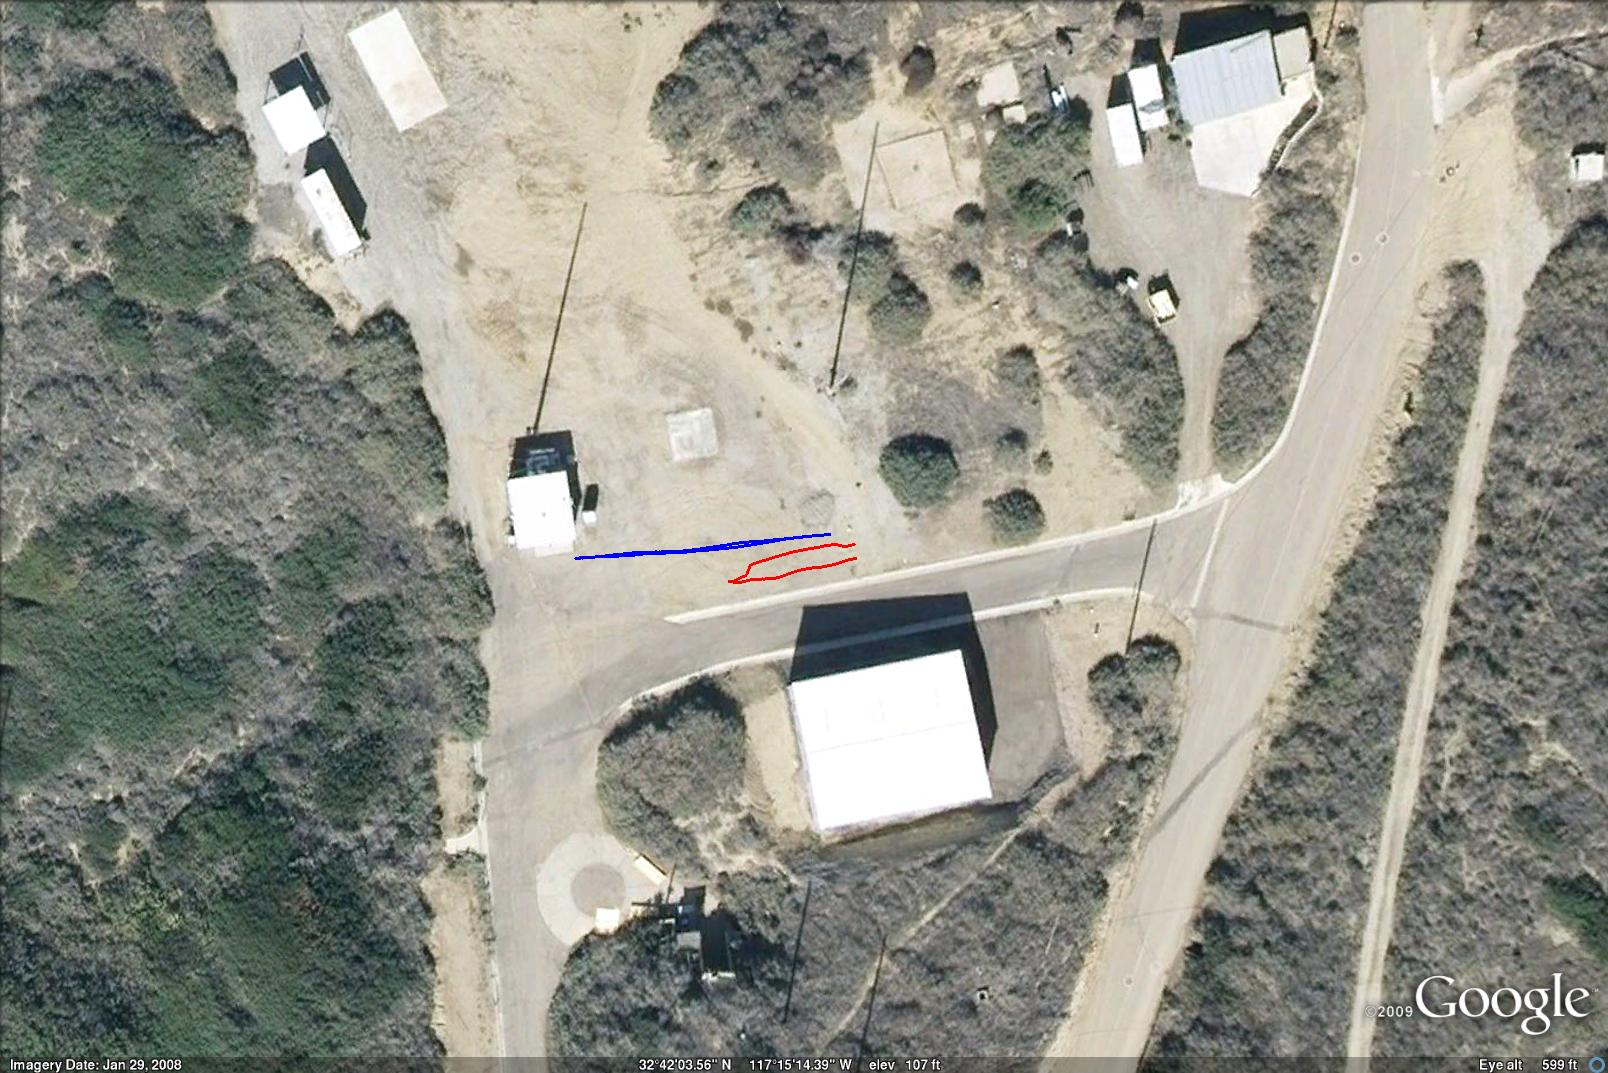
\includegraphics[width=.7\textwidth]{images/GE/GEHeadingReverseFixed}
%	\caption{Route Driven by PackBot to Test Heading}
%	\label{fig:GEHeadingReverse}
%\end{figure}
%
%\begin{figure}[ht!]
%	\centering
%	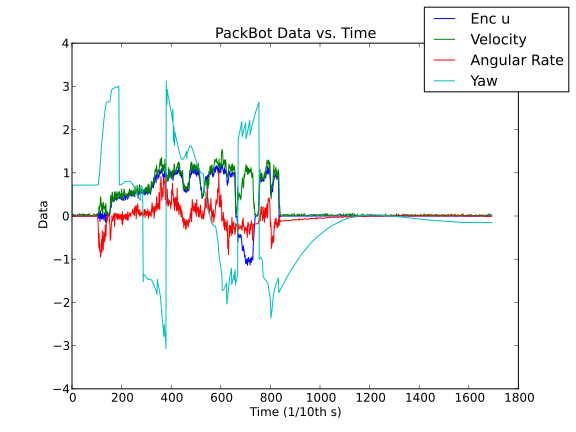
\includegraphics[width=.7\textwidth]{images/pbDataReverseHeading}
%	\caption{Heading and Velocity Reversed}
%	\label{fig:pbDataReverseHeadingBroken}
%\end{figure}
%
%\begin{figure}[ht!]
%	\centering
%	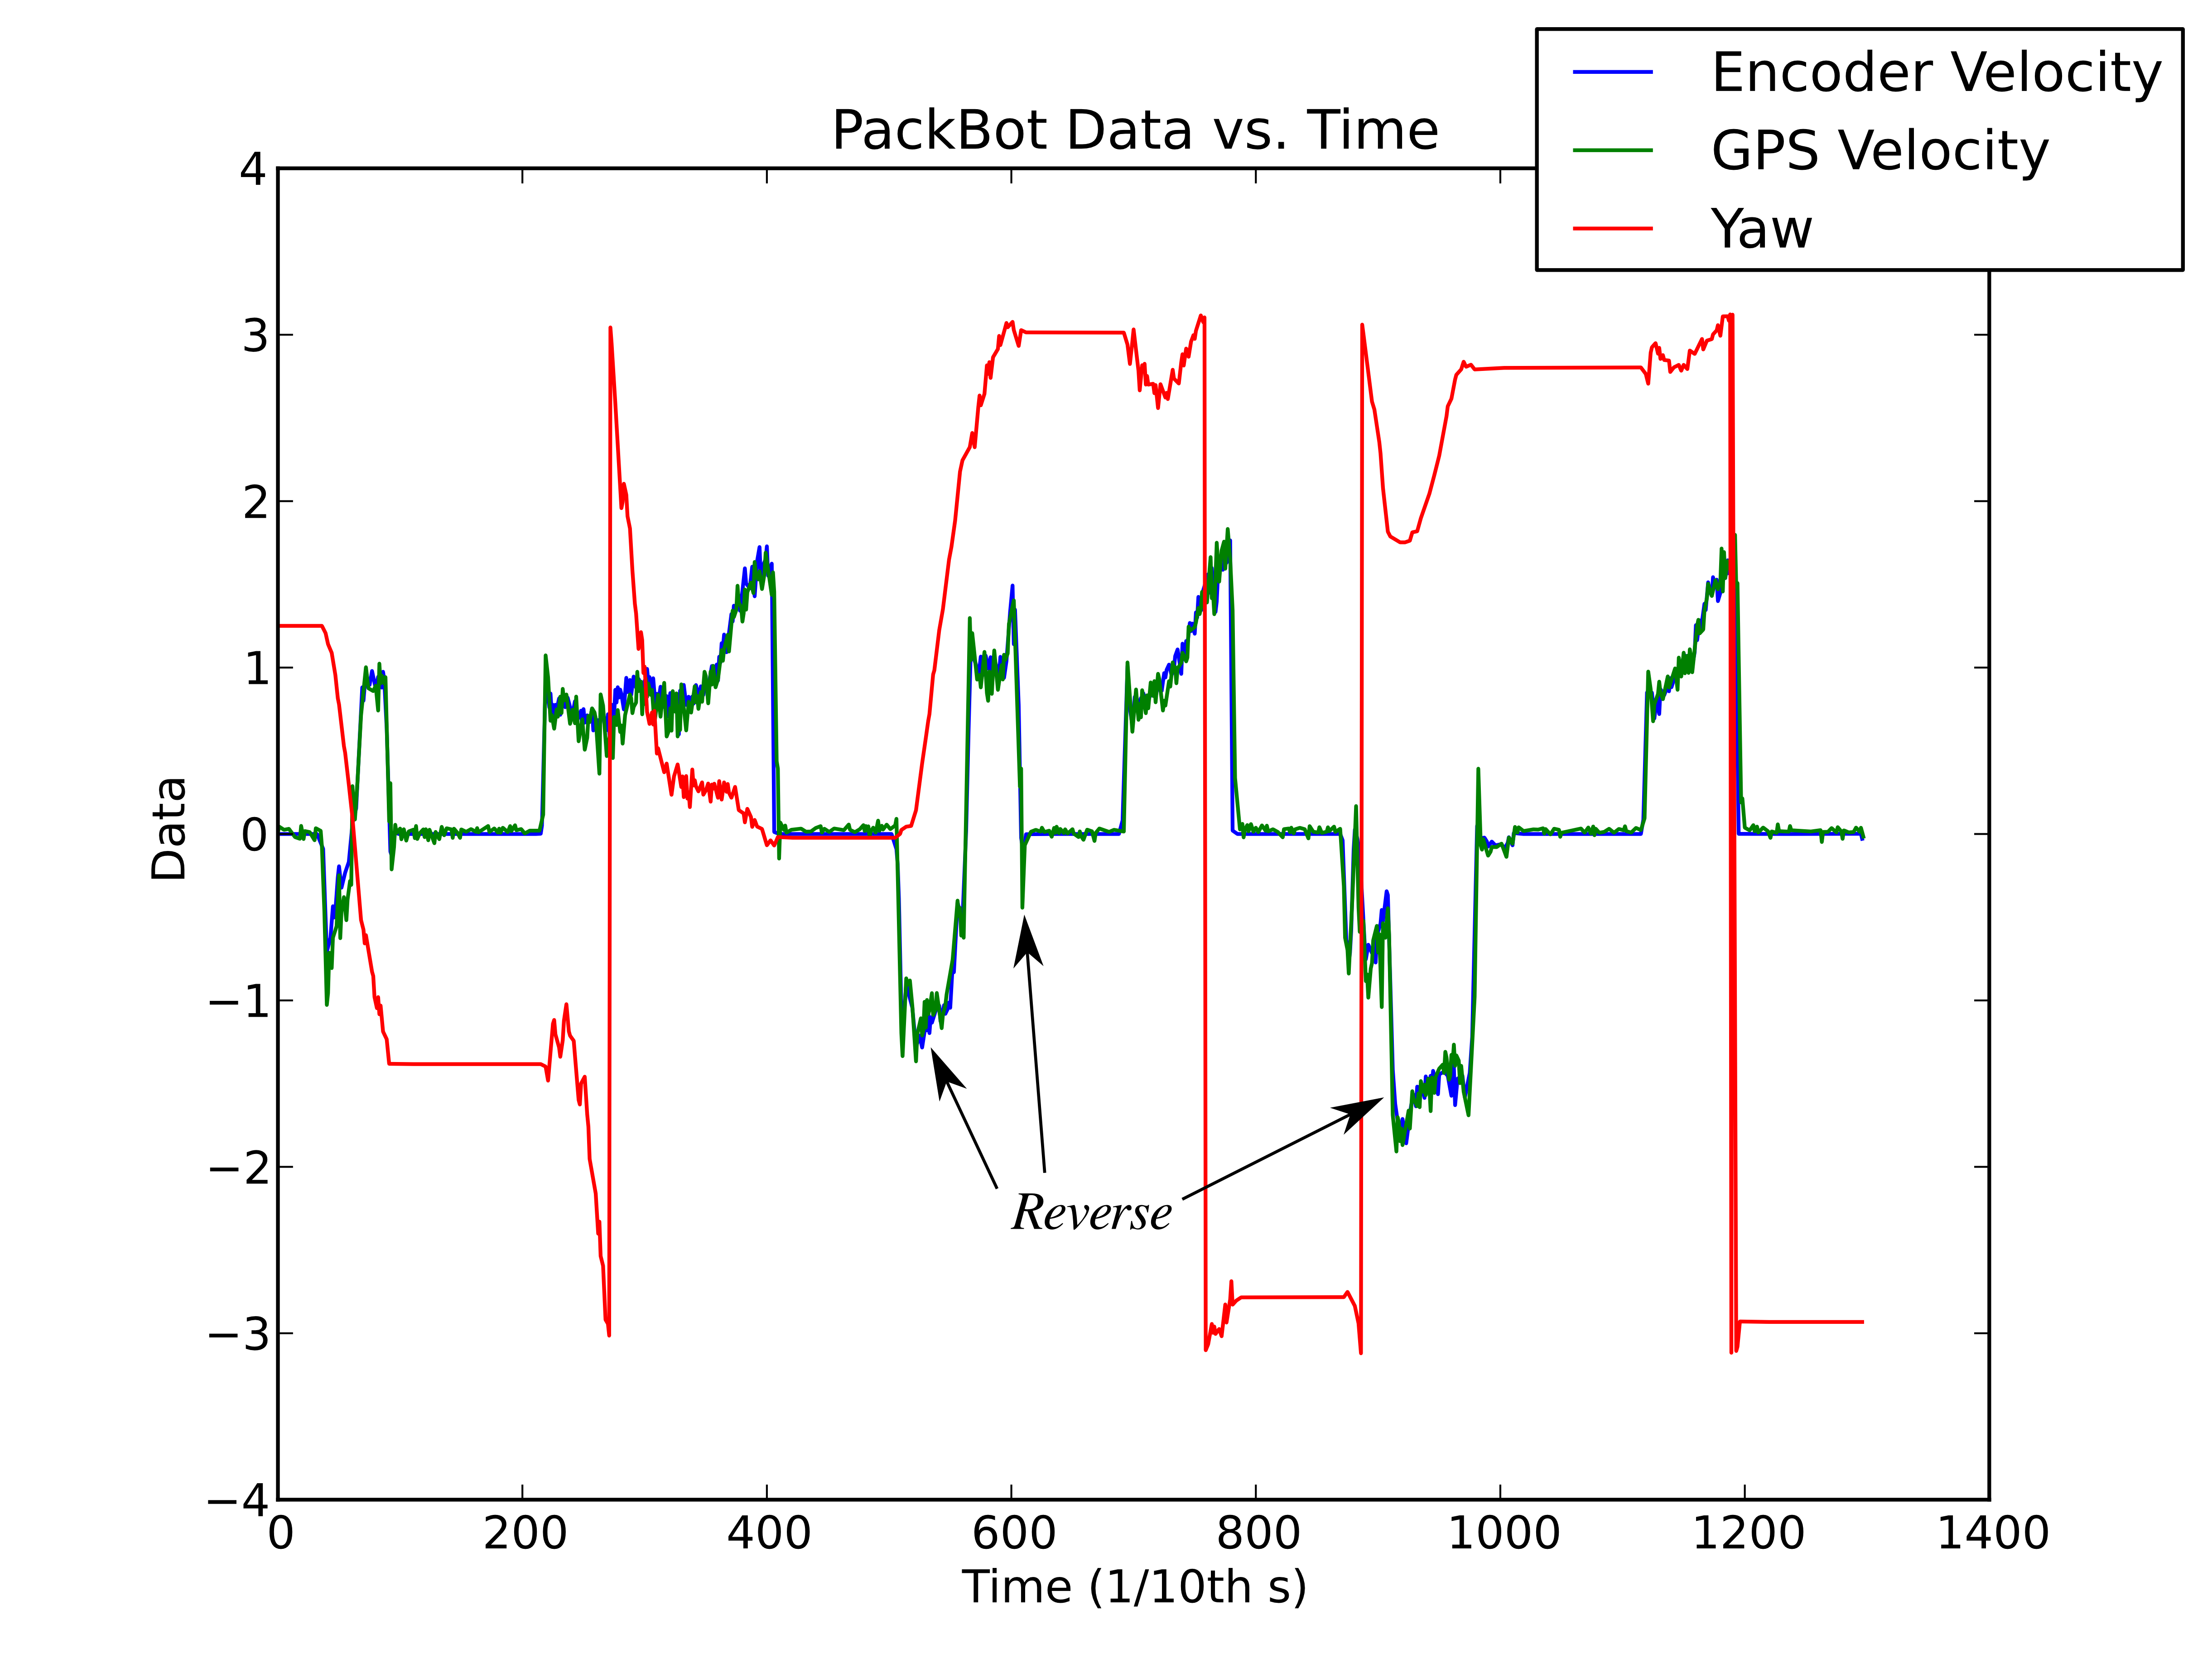
\includegraphics[width=.7\textwidth]{images/KFDataHeadingReverseFixed}
%	\caption{Heading Fixed When Driving in Reverse}
%	\label{fig:pbDataReverseHeadingFixed}
%\end{figure}

\section{Fixing Bugs in ACS Kalman Filter}
\label{sec:kfBugs}
The ACS Kalman filter contained three major bugs in the equations and only worked because of a reforumlation of the standard Kalman filter equations. The first bug concerned the calculation of the Kalman gain matrix (see Chapter \ref{kfKalmanGain}). The $K_k$ matrix was being calculated correctly but at the end of the calculation gains from previous sensors were added back into their former element locations in the matrix. This bug was fixed by removing the code that added previous gain elements back into the Kalman gain matrix. One of the consequences of this bug is that the calculation of the covariance of the state estimate in the prediction update step used the continuous time system model $F$ (\ref{eq:kfjacobianresult}) instead of the discrete time system model $\Phi_k$ (\ref{eq:kfSystemModelWithAssumptions}) such that instead of $P_{k+1}^- = \Phi_kP_k^-\Phi_k^T + Q_k$ (c.f. (\ref{eq:kfpredictionupdate})) the Kalman filter used

\begin{align*}
P_{k+1}^- = FP_k^+F^T + Q_k.
\end{align*}
The discrete time system model $\Phi_k$ was used in the calculation of the state estimate $\hat{x}_k^-$ though. After this fix the discrete time system model was used appropriately in the state covariance calculation during the prediction update step.

The second bug was a consequence of calculating the Kalman gain incorrectly. The yaw angle calculation was not being done correctly since the state covariance estimate was wrong so a correcting term was introduced that fixed the yaw angle when the standard set of sensors were used since they reliably gave measurements at a fixed rate and affected the Kalman gain matrix in a consistent manner. This bug was also fixed by simply removing the correcting term and the yaw angle was estimated correctly after the Kalman gain matrix was implemented properly.

The third bug was slightly less significant but still posed several problems. In the measurement update step (\ref{eq:kfmeasurementupdate}) the measurement model $H_k$ was set up to use the latest received data from each sensor at each time step rather than only use new measurements if they were available from each sensor. This bug manifested itself most prominently in sensors with slow update rates such as GPS. One particular robot configuration used a GPS receiver that output position fixes at $1 Hz$ which resulted in the Kalman filter measurement update (running at $100 Hz$) using the same position measurement for $100$ time steps when that particular measurement should only have been used a single time out of the $100$ time steps. This became obvious when the control system exhibited the behavior of cycling through slowing down and speeding up in a very jerky fashion. This occurred because the Kalman filter was trying to push the position estimate backwards toward the most recent GPS measurement instead of letting the system model $\Phi_k$ allow the robot position to propagate forward based on the robot kinematics.

\section{Establishing Ground Truth}
\label{sec:groundtruth}
Quantitatively evaluating the performance of Kalman filters can be accomplished in several ways, the best of which is to analyze the output of the Kalman filter against ground truth. Although it is nearly impossible to establish ground truth over a large area in practice the closer the measurements are to an absolute position in the world the better. To determine ground truth for the robots in these experiments a differential GPS (DGPS) system was used independently of the sensors on the robot so that very accurate measurements of the robots actual position could be logged and then used in a post-processing step to determine how well the Kalman filter estimate corresponds to ground truth.

The DGPS system consists of a GPS receiver and serial radio that make up the base station and a GPS receiver, serial radio and small computer that make up the roaming station as in Figure \ref{fig:dgps}. The GPS receivers are both Novatel receivers using the Real Time Kinematics algorithm. The base station is located in a static position and is configured to use a fixed position which is compared to what the current position would be if it were not fixed. The difference between the fixed position and the calculated position are used to generate corrections that would put the position of the GPS antenna at the fixed position and those corrections are sent to and applied at the roaming station resulting in a standard deviation of $2$ $cm$ for the position output of the roaming station. The errors are due to the effects of the GPS signal passing through the atmosphere from the satellites to the antenna as well as to multipath effects closer to the ground. The DGPS corrections are used for each satellite that the ground station and the roaming station share in the constellation of satellites they are using in their solution of a position estimate. The DGPS system is bootstrapped to the robot during testing runs to log data at a rate of $10$ $Hz$ and is only used as a tool to measure ground truth for position and is not meant to be used during normal operation.

With a highly accurate estimate of ground truth established it becomes possible to not only study the performance of the Kalman filter but to also begin determining whether to focus efforts in improving the autonomous navigation behaviors of the robots via the estimation or controls algorithms.

\begin{figure}[ht!]
	\centering
	\includegraphics[width=.6\textwidth]{images/dgps}
	\caption{Differential GPS System Diagram}
	\label{fig:dgps}
\end{figure}

\section{Identifying Noise Models}
\label{sec:kfIdentifyNoiseModels}
Attempting to determine the proper values for the noise models $Q_k$ in (\ref{eq:kfpredictionupdate}) and $R_k$ in (\ref{eq:kfmeasurementupdate}) can be a laborious process and is often considered more of an art than a science with engineer experience being a critical factor. In Chapter \ref{sec:kfNoiseModels} it was shown that the Kalman filter performance is heavily dependent upon the accuracy of the noise models even though they are difficult to determine. Several methods exist to assist engineers in determining proper relative weighting of the elements in $Q_k$ and $R_k$ to improve Kalman filter performance after initial values are selected by the engineer.

%\subsection{Adaptive Extended Kalman Filter}
%\label{sec:adaptiveekf}
%*** Why is it valid to update $Q_k$ and $R_k$ this way? Talk about how the updates are turned off when the velocity is zero, otherwise $Q_k$ and $R_k$ are adapted to a static, not dynamic, state. Similarly, talk about how this method doesn't work as well as would be hoped because the original application was for tracking satellites with low dynamics and robots have high dynamics, especially when navigating around obstacles. Also, look at the extra stuff that Busse says he had to do to get this algorithm to work in practice. I say high dynamics here, but what about the low dynamics assumption? Low is relative to sensor noise and satellites have much higher quality sensors so the noise level is much lower in addition to the actual dynamics being lower. ***
%
%In order to improve the noise models the ACS Kalman filter has been implemented with an adaptive scheme to update the covariance matrices $Q_k$ and $R_k$ in real time as the robot moves around and sensor measurements are taken into account to help overcome the time intensive nature of determining these matrices and add a degree of robustness to the state estimate \cite{Sights06}, \cite{Mehra72}, \cite{Busse03adaptiveEKF}. Estimates of $Q_k$ and $R_k$ are updated at alternating time steps in the EKF. Recall from (\ref{eq:kfpredictionupdate}) and (\ref{eq:kfmeasurementupdate}) that $\hat{x}_k^+$ and $P_k^+$ are known after the measurement update step and $\hat{x}_k^-$ and $P_k^-$ are known after the system update step in the Kalman filter.
%
%As shown in \cite{Busse03adaptiveEKF} the first step is to calculate $Q^\star$ using
%\begin{align*}
%% \label{eq:qstar}
%Q^\star = \left(\hat{x}_k^+-\hat{x}_k^-\right)\left(\hat{x}_k^+-\hat{x}_k^-\right)^T + P_k^- - P_k^+ - \hat{Q}_k^-.
%\end{align*}
%Then the estimate of $Q_k$ is updated such that
%\begin{align}
%\label{eq:qadapt}
%\hat{Q}_k^+ = \hat{Q}_k^- + \frac{1}{L_Q}\left(Q^\star-\hat{Q}_k^-\right).
%\end{align}
%
%Next $R^\star$ is calculated using
%\begin{align*}
%% \label{eq:rstar}
%R^\star = \left(y_k-\hat{y}_k^+\right)\left(y_k-\hat{y}_k^+\right)^T - H_kP_k^+H_k^T
%\end{align*}
%where $y_k$ are actual measurement data and $\hat{y}_k^+ = h_k\hat{x}_k^+$ is calculated after the measurement update step. Then the estimate of $R_k$ is updated such that
%\begin{align}
%\label{eq:radapt}
%\hat{R}_k^+ = \hat{R}_k^- + \frac{1}{L_R}\left(R^\star-\hat{R}_k^-\right).
%\end{align}
%It can be seen that the estimates of both covariance matrices employ a running average algorithm and vary the weight of recent measurements and state updates via the adaptation coefficients $L_Q$ and $L_R$.

\subsection{Discriminative Training of Kalman Filter Parameters}
\label{sec:kftrainingparams}
A method to automatically learn what the covariance matrices $Q_k$ and $R_k$ that make up the noise models in the Kalman filter should be by using a discriminative training algorithm was described in \cite{Abbeel-RSS-05}. Building upon that work \cite{SakaiKuroda10} recently used a variation of the algorithm described in \cite{Abbeel-RSS-05} to learn parameter values for the noise filters used in their unscented Kalman filter. This method takes advantage of ground truth measurements obtained using a DGPS system like that described in Chapter \ref{sec:groundtruth}. Note that in the following expressions the term $h(\mu_t)$ is the position output by the Kalman filter and $y$ is the DGPS position output so the goal is to find values of $Q_k$ and $R_k$ that minimize the difference between the output of the Kalman filter and DGPS ground truth.

There are several metrics that can be applied to the data with the two most relevant metrics being the residual error metric and the prediction likelihood error metric. The residual prediction error is used to estimate $Q_k$ and $R_k$ using
\begin{align*}
\left<R_{\text{res}},Q_{\text{res}}\right> = \argmin_{R,Q}\sum_{t=0}^T ||y_t-h(\mu_t)||_2^2.
\end{align*}
When the covariance matrix $P$ for the ground truth sensor is \textit{not} a multiple of the identity matrix $I$ then this metric is
\begin{align*}
\left<R_{\text{res}},Q_{\text{res}}\right> = \argmin_{R,Q}\sum_{t=0}^T (y_t-h(\mu_t))^TP^{-1}(y_t-h(\mu_t)).
\end{align*}
The error metric used for the residual prediction error method is
\begin{align}
\label{eq:kftrainingres}
e = \left(\frac{1}{T}\sum_{t=1}^T ||h(\mu_t)-y_t||^2\right)^{1/2}.
\end{align}

The prediction likelihood method use the metric
\begin{align*}
\left<R_{\text{pred}},Q_{\text{pred}}\right> = \argmax_{R,Q}\sum_{t=0}^T -\log|2\pi\Omega_t| - (y_t-h(\mu_t))^T\Omega_t^{-1}(y_t-h(\mu_t))
\end{align*}
where $\Omega_t = H_t\Sigma_tH_t^T+P$. The error metric used for the prediction likelihood method is
\begin{align}
\label{eq:kftrainingpred}
e = -\frac{1}{T}\sum_{t=1}^T \left(\log|2\pi\Omega_t| - (y_t-h(\mu_t))^T\Omega_t^{-1}(y_t-h(\mu_t))\right)
\end{align}
where $\Omega_t$ is the same as in the above description.

\subsection{Simulating Robot Runs}
\label{sec:kfSimulation}
For the training algorithm to work the sensor data collected from a robot has to be replayed a large number of times. To accomplish this a simulation of the robot that runs faster than real time run helps to reduce the amount of time taken to replay the data when using the candidate noise models so that the results can be evaluated. As shown in Table \ref{tab:kfSimulationErrors} the position errors as calculated using (\ref{eq:kftrainingres}) were very close between the simulated runs and the actual robot run. The average error was $0.0556~m$ over nine different runs which gives a baseline for the convergence criterion. The best that the training program can do is converge to an error approximately equal to the average error of the simulation compared to actual data.

\begin{table}[ht!]
\caption{Kalman Filter Simulation Errors}
\small
\centering
\begin{tabular}{@{}lllr@{}} \toprule
Run & Actual Error (m)  & Simulation Error (m) & Error Difference (m) \\ \midrule
1   & 0.452886          & 0.423056             & 0.029830             \\
2   & 0.177620          & 0.210472             & 0.032852             \\
3   & 0.109484          & 0.080400             & 0.029084             \\
4   & 0.494375          & 0.491243             & 0.003132             \\
5   & 0.068306          & 0.035943             & 0.032363             \\
6   & 0.000028          & 0.105102             & 0.105074             \\
7   & 0.017564          & 0.033453             & 0.015889             \\
8   & 2.599853          & 2.427348             & 0.172505             \\
9   & 0.020686          & 0.100696             & 0.080010             \\ \bottomrule
\end{tabular}
\label{tab:kfSimulationErrors}
\end{table}

\subsection{Coordinate Ascent Algorithm}
\label{sec:coordinateAscent}
In order to evaluate the error metrics in (\ref{eq:kftrainingres}) and (\ref{eq:kftrainingpred}) it is necessary to search through the space of parameters to find the optimal parameters to use in the $Q_k$ and $R_k$ matrices. Initially, a program was written to attempt a naive, brute force approach of trying every possible combination of parameters. The brute force algorithm turned out to be difficult to implement, took several days to run and returned unimpressive results that did not really improve the Kalman filter estimates. Following the description in \cite{Abbeel-RSS-05} a coordinate ascent algorithm was then written with much better results and faster convergence times.

The coordinate ascent algorithm was initialized by a set of hand-tuned noise model parameters and then the robot run was simulated. For each parameter in the noise models the value of the parameter is then increased by $\alpha_i \%$ and the error metric is evaluated. If the resulting error is less than the previous best result the parameter is kept at the increased value, otherwise the parameter is decreased by $\alpha_d \%$. The values $\alpha_i$ and $\alpha_d$ are known as the learning rates. One iteration of the algorithm consists of running the simulation and evaluating the error metric for each of the noise parameters and the algorithm continues until the error is less than some convergence value $\epsilon$ or until two consecutive iterations are run without producing a new minimum error.

Essentially the training algorithm trades tuning the actual noise parameters in the $Q_k$ and $R_k$ matrices for tuning the learning rate parameters $\alpha_i$ and $\alpha_d$.
